
This three-dimensional benchmark was first proposed by \cite{bucc93}. 
It has been subsequently presented in \cite{tack94,trha98,albe00,omma06,dawk11,krhb12}.
We here focus on Case 1 of \cite{bucc93}:  an isoviscous bimodal convection experiment at $Ra=3\times 10^5$.

The domain is of size $a\times b\times h$ with $a=1.0079h$, $b=0.6283h$ with $h=2700$km. It is filled with a Newtonian fluid
characterised by $\rho_0=3300{\rm kg}.{\rm m}^{-3}$, $\alpha=10^{-5}{\rm K}^{-1}$, $\mu=8.0198\times10^{23}{\rm Pa.s}$, 
$k=3.564{\rm W}.{\rm m}^{-1}.{\rm K}^{-1}$, 
$c_p=1080{\rm J}.{\rm K}^{-1}.{\rm kg}^{-1}$.
The gravity vector is set to ${\bm g}=(0,0,-10)^T$.
The temperature is imposed at the bottom  ($T=3700^\circ$C) and at the top ($T=0^\circ$C).

The various measurements presented in \cite{bucc93} are listed hereafter:
\begin{itemize}
\item The Nusselt number $Nu$ computed at the top surface following Eq. (\ref{eqNu}):
\[
Nu = L_z \frac{\int\int_{z=L_z} \frac{\partial T}{\partial y} dx dy  }{\int \int_{z=0} T dx dy}
\]
\item the root mean square velocity $v_{rms}$ and the temperature mean square velocity $T_{rms}$
\item The vertical velocity $w$ and temperature $T$ at points ${\bm x}_1=(0,0,L_z/2)$, ${\bm x}_2=(L_x,0,L_z/2)$,
${\bm x}_3=(0,L_y,L_z/2)$ and ${\bm x}_4=(L_x,L_y,L_z/2)$;
\item the vertical component of the heat flux $Q$ at the top surface  at all four corners.
\end{itemize}

The values plotted hereunder are adimensionalised by means of a reference temperature (3700K),
a reference lengthscale 2700km, and a reference time $L_z^2/\kappa$. 

\begin{center}
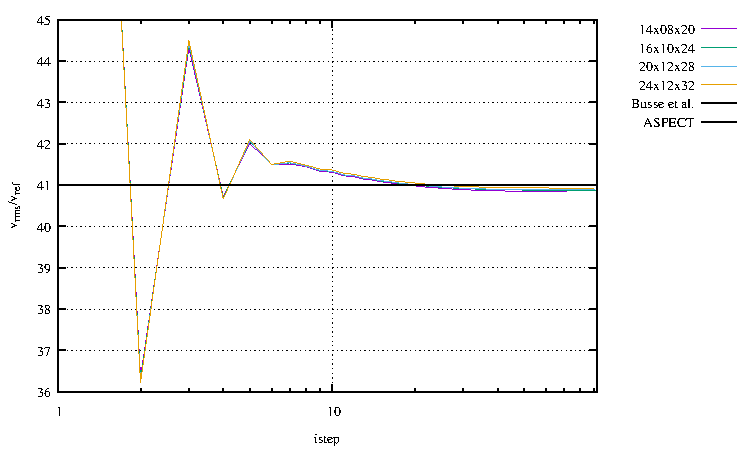
\includegraphics[width=8cm]{python_codes/fieldstone_20/results/vrms.pdf}
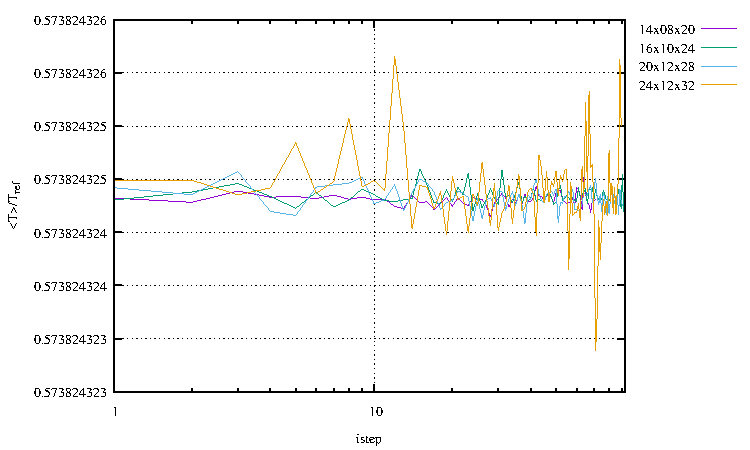
\includegraphics[width=8cm]{python_codes/fieldstone_20/results/Tavrg.pdf}\\
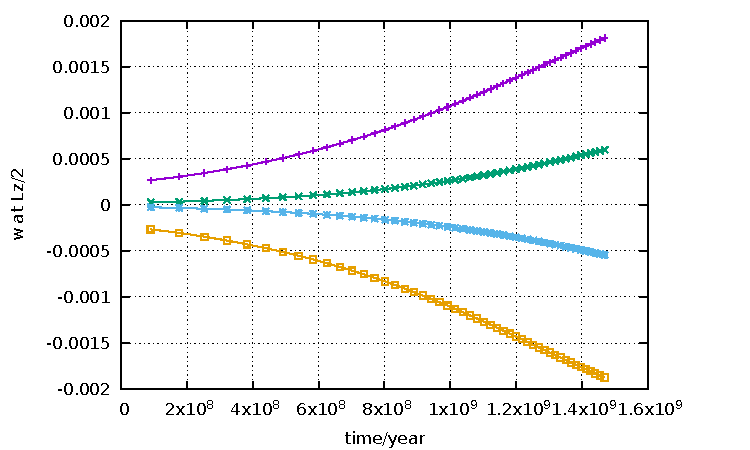
\includegraphics[width=8cm]{python_codes/fieldstone_20/results/wmid.pdf}
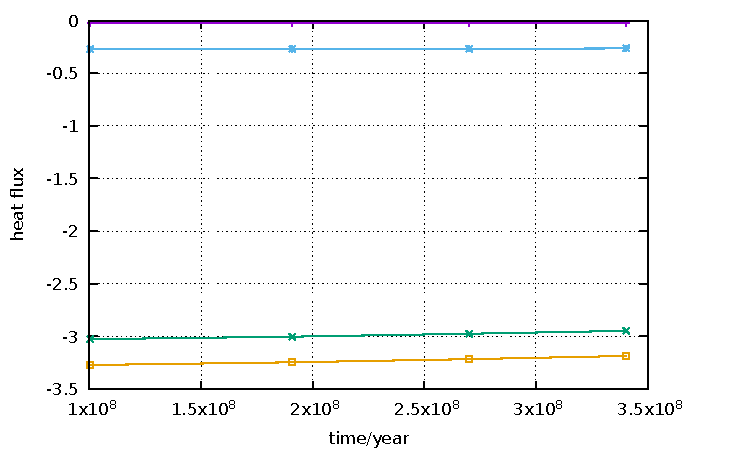
\includegraphics[width=8cm]{python_codes/fieldstone_20/results/hf.pdf}
\end{center}


\fbox{
\parbox{10cm}{{\bf features}
\begin{itemize}
\item $Q_1\times P_0$ element
\item incompressible flow
\item mixed formulation
\item Dirichlet boundary conditions (free-slip)
\item direct solver
\item isothermal
\item non-isoviscous
\item 3D
\item elemental b.c. 
\item buoyancy driven
\end{itemize}
}}

{\color{red} ToDo}: look at energy conservation. run to steady state and make sure the expected values are retrieved.

